\documentclass[11pt,a4paper]{article}

% Idioma y codificación
\usepackage[utf8]{inputenc}
\usepackage[T1]{fontenc}
\usepackage[spanish,es-tabla]{babel}

% Formato de página
\usepackage[a4paper, margin=2.5cm]{geometry}
\usepackage{setspace}
\onehalfspacing

% Matemáticas
\usepackage{amsmath, amssymb, amsfonts, amsthm}
\usepackage{bm}
\usepackage{mathtools}

% Figuras y tablas
\usepackage{graphicx}
\graphicspath{{figures/}}
\usepackage{float}
\usepackage{booktabs}
\usepackage{multirow}
\usepackage{caption}
\usepackage{subcaption}
\usepackage{tabularx}   % Tablas con ancho ajustable

% Bibliografía
\usepackage{csquotes}
\usepackage[backend=biber, style=ieee]{biblatex}
\addbibresource{ref.bib}

% Enlaces (hyperref casi siempre al final)
\usepackage[
    colorlinks=true,
    linkcolor=black,
    citecolor=blue,
    urlcolor=blue
]{hyperref}

% ====================== INFORMACIÓN DEL DOCUMENTO ===========================
\newcommand{\Titulo}{
    Colapso en Mamba y en Modelos de Espacio de Estados Selectivos
}

\newcommand{\Autores}{
    Raquel Fernández Esquinas\\
    Isabel V. Morell Maudes
}

\newcommand{\Universidad}{
    Universidad Pontificia Comillas\\
    Escuela Técnica Superior de Ingeniería (ICAI)
}

\newcommand{\Asignatura}{
    Métodos Diferenciales de la Inteligencia Artificial
}

\newcommand{\fecha}{
    Noviembre, 2026
}

\hypersetup{
    pdftitle={Colapso en Mamba y en Modelos de Espacio de Estados Selectivos},
    pdfauthor={Fernández, Morell}
}

\begin{document}

% ====================== PORTADA ===========================
\begin{titlepage}
    \centering
    \vspace*{1.5cm}
    % Logo de la universidad (opcional)
    
\includegraphics[width=0.3\textwidth]{figures/logo.png}

    \vspace{1.5cm}
    {\Large \Universidad\par}

    \vspace{2.5cm}
    {\Huge \bfseries \Titulo\par}

    \vspace{2cm}
    {\large
        \textbf{Autores}\\[0.4cm]
        \Autores
    }

    \vfill
    {\large
        \textbf{\Asignatura}\\[0.3cm]
        \fecha
    }
    \vspace{1cm}
\end{titlepage}

% ====================== CAPÍTULOS ===========================
% ============================================================================
% 1. Introducción y recordatorio de self-attention
% ============================================================================
\section{Introducción}
\label{sec:intro}

Los modelos basados en \textit{Transformers} alcanzan un alto rendimiento en el procesamiento de secuencias, 
aunque su coste computacional aumenta considerablemente con la longitud de estas. Como alternativa, han 
surgido arquitecturas basadas en modelos de espacio de estados (\textit{State Space Models}, SSMs), que 
permiten procesar secuencias largas más eficientemente. Sin embargo, los SSMs tradicionales presentan 
limitaciones para seleccionar dinámicamente la información relevante en secuencias como las del lenguaje natural.

Para abordar esta limitación, Gu y Dao \cite{gu2023mamba} introdujeron Mamba, una arquitectura que incorpora 
un mecanismo de selección dependiente de la entrada. Este permite adaptar los parámetros en cada posición de 
la secuencia, controlando así qué información se incorpora al estado oculto y cuál se conserva del estado 
anterior.

En este trabajo, analizamos la dinámica de los tokens en Mamba a partir del estudio de Vo et al. \cite{vo2025token}. 
En particular, estudiamos los fenómenos de convergencia y divergencia de las representaciones, 
así como las condiciones y los factores que determinan su comportamiento.
\newpage
% ============================================================================
% 2. SSM continuo, discretización y qué hace "selectivo" a Mamba
% Responsable: Isabel
% Prefijo de etiquetas: sec:ssm-, fig:ssm-, eq:ssm-, thm:ssm-
% ============================================================================
\section{Modelos de espacio de estados selectivos}
\label{sec:ssm}

\subsection{El SSM continuo}
\label{sec:ssm-continuo}

\todo{Sistema lineal $h'(s)=A h(s)+B x(s)$, $y(s)=C h(s)$; interpretación de $h$, $A$, $B$, $C$.}

\subsection{Discretización}
\label{sec:ssm-discretizacion}

\todo{Paso $\Delta$, discretización de $A$ y $B$ y recursión resultante. Dejar claro qué discretización usa Mamba y cuál se simplifica en el modelo de \cite{vo2025token}.}

\subsection{Qué hace selectivo a Mamba}
\label{sec:ssm-selectivo}

\todo{$B$, $C$ y $\Delta$ dependen de la entrada: $\Delta_d(u)=\softplus(S_{\Delta,d}\,u)$, $B=\SB x$, $C=\SC x$, con $\SB,\SC\in\R^{\estado\times D}$.}

\subsection{Límite continuo en profundidad}
\label{sec:ssm-limite}

\todo{Cómo se llega a la EDO de tokens (solo capa S6 y conexión residual, con la profundidad como tiempo). Esta subsección es el puente hacia la sección~\ref{sec:dinamica}; \todo{Raquel la lee con cuidado}.}

% Con A_d = -a_d I, la dimensión de estado N solo entra en la dinámica a través
% de M = S_C^T S_B (rango <= N). Esto es lo que usa la sección 4.1.
\begin{observacion}\label{obs:ssm-rango}
  Con $A_d=-a_d I$, la dimensión de estado $\estado$ interviene en la dinámica solo a través de $\Mmat=\SC\transp\SB\in\R^{D\times D}$, cuyo rango es como mucho $\min(\estado,D)$.
\end{observacion}

\newpage
% ============================================================================
% 3. Dinámica de tokens: resultados del paper y tasas desiguales
% Responsable: Raquel
% Prefijo de etiquetas: sec:din-, fig:din-, eq:din-, thm:din-
% Las simulaciones que ilustran estos resultados van en secciones/04*.tex.
% ============================================================================

% Entorno de teoremas: solo se define si el preámbulo no lo ha definido ya.
\makeatletter
\@ifundefined{teorema}{\newtheorem{teorema}{Teorema}[section]}{}
\makeatother

\section{Dinámica de tokens}
\label{sec:dinamica}

\subsection{La EDO de tokens}
\label{sec:din-edo}

Para estudiar qué ocurre con los tokens al atravesar muchas capas, seguimos a \cite{vo2025token} y partimos de la recurrencia de la sección~\ref{sec:ssm}. Al eliminar el estado oculto $h_{dl}$, la salida de cada canal pasa a ser una combinación lineal de los tokens anteriores,
\begin{equation}
  y_{dl}=\sum_{j=1}^{l}P_{dlj}\,x_{dj},
  \label{eq:din-salida}
\end{equation}
donde $P_d$ es una matriz triangular inferior cuyas entradas son
\begin{equation}
  P_{dlj}=
  \begin{cases}
    x_l^{\top}M\,x_l\;\Delta_d(x_l), & j=l,\\[4pt]
    x_l^{\top}M\,x_j\;\Delta_d(x_j)\,\exp\!\Big(-a_d\displaystyle\sum_{k=j+1}^{l}\Delta_d(x_k)\Big), & j<l,
  \end{cases}
  \label{eq:din-P}
\end{equation}
y $M=S_C^{\top}S_B$ es la matriz de entrada-salida. Los autores llaman a $P$ \emph{atención oculta} por su parecido con la matriz de atención: pondera cada token con los anteriores y es causal. Sin embargo, a diferencia de la atención, sus filas no están normalizadas y sus entradas no tienen por qué ser positivas.

Para pasar al continuo interpretamos el índice de capa como un tiempo $t\in[0,\infty)$ y conservamos únicamente la capa S6 y la conexión residual, de la misma forma que se hace con las ResNets y los Transformers (sección~\ref{sec:ssm-limite}). De esta forma obtenemos la EDO de tokens
\begin{equation}
  \frac{\mathrm{d}x_{dl}}{\mathrm{d}t}(t)=\sum_{j=1}^{l}P_{dlj}(t)\,x_{dj}(t),
  \qquad x_{dl}(0)=x_{dl0}\in\mathbb{R},
  \label{eq:din-edo}
\end{equation}
donde $P_{dlj}(t)$ se define como en \eqref{eq:din-P} evaluando los tokens en $x(t)$.

Este modelo es una simplificación de Mamba: se ignoran la normalización de capa, la convolución y las capas lineales, y se supone que los parámetros $A_d$, $S_{\Delta,d}$, $S_B$ y $S_C$ no dependen de $t$. Los autores lo justifican por conveniencia matemática, y señalan que en la práctica se comparten pesos entre capas. Por ello, los resultados que siguen describen este modelo simplificado y no la arquitectura completa.

\subsection{Caso unidimensional}
\label{sec:din-1d}

Con un solo canal ($D=1$), la matriz $M$ es un escalar que denotamos $\mu=S_C^{\top}S_B$, y $\Delta(u)=\mathrm{softplus}(S_\Delta u)$. Suponemos $x_{l0}\neq 0$ para todo $l$, para evitar el caso trivial. Para $l=1$ la EDO \eqref{eq:din-edo} se reduce a una ecuación autónoma,
\begin{equation}
  \dot{x}_1=\mu\,x_1^{3}\,\Delta(x_1),
  \label{eq:din-token1}
\end{equation}
y los demás tokens se acoplan al primero a través de $P$. El signo de $\mu$ y el de $S_\Delta x_{l0}$ determinan tres escenarios, que recogen los siguientes resultados de \cite{vo2025token}.

\begin{teorema}[Convergencia]\label{thm:din-conv}
  Si $\mu<0$, para cada $l$ se cumple que, si $x_{l0}>0$ (resp. $<0$), $x_l(t)$ es positiva y decreciente (resp. negativa y creciente). Además, $x_l(t)=O(1/\sqrt{t})$ y $P_{lj}(t)=O(1/t)$ para todo $l,j$.
\end{teorema}

\begin{teorema}[Divergencia lenta]\label{thm:din-lenta}
  Si $\mu>0$ y $S_\Delta x_{L0}\le\cdots\le S_\Delta x_{10}\le -2{,}12$, para cada $l$ se cumple que, si $x_{l0}>0$ (resp. $<0$), $x_l(t)$ es positiva y creciente (resp. negativa y decreciente). Además, $x_l(t)=O\big((\ln t)^{l}\big)$ y $P_{lj}(t)\to 0$ cuando $t\to\infty$, para todo $l\ge j$.
\end{teorema}

\begin{teorema}[Divergencia rápida]\label{thm:din-rapida}
  Si $\mu>0$ y existe algún $l$ con $S_\Delta x_{l0}>0$, entonces $x_l(t)$ diverge en tiempo finito. Además, si $x_{l^*}$ es el primer token en divergir, en un instante $T$, y el resto de tokens están definidos en $[0,T]$, entonces $\lim_{t\to T^-}P_{lj}(t)=+\infty$ si y solo si $l=l^*$ o $j=l^*$, para $L\ge l\ge j\ge 1$.
\end{teorema}

En el apéndice del paper la constante $-2{,}12$ de la divergencia lenta se afina a $-r_0$, con $r_0\approx 2{,}116$. En resumen, para $D=1$ los tokens convergen todos a cero ($\mu<0$) o divergen todos a infinito ($\mu>0$), y en este último caso lo hacen despacio o en tiempo finito según el signo de $S_\Delta x_{l0}$. La Figura~\ref{fig:param-escenarios} muestra los tres escenarios.

La ecuación \eqref{eq:din-token1} permite además precisar la tasa del primer token en el caso convergente. Por el Teorema~\ref{thm:din-conv}, $x_1(t)\to 0$, y por tanto $\Delta(x_1)\to\Delta(0)=\ln 2$. Como
\[
  \frac{\mathrm{d}}{\mathrm{d}t}\,x_1^{-2}=-2x_1^{-3}\dot{x}_1=2|\mu|\,\Delta(x_1)\longrightarrow 2|\mu|\ln 2,
\]
resulta que $\sqrt{t}\,|x_1(t)|\to(2|\mu|\ln 2)^{-1/2}$. Este cálculo es nuestro y no aparece en el paper; lo comprobamos numéricamente en la Figura~\ref{fig:param-tasas}, donde para $\mu=-1$ el límite es $0{,}849$.

\subsection{Tasas desiguales}
\label{sec:din-tasas}

Los tres escenarios se diferencian también en cómo se reparten las tasas entre las posiciones de la secuencia:
\begin{itemize}
  \item \textbf{Convergencia.} Todos los tokens decaen con la misma tasa, $O(1/\sqrt{t})$, y la atención oculta como $O(1/t)$. Sin embargo, la constante depende de la posición: en el ejemplo de la Figura~\ref{fig:param-tasas}, $\sqrt{t}\,|x_l|$ se estabiliza en $0{,}849$ para el primer token y en $0{,}60$ para el resto.
  \item \textbf{Divergencia lenta.} La cota $(\ln t)^{l}$ crece con la posición $l$, de forma que los tokens más tardíos pueden crecer mucho más que los primeros. Según los autores, los tokens con mayor valor absoluto divergen más rápido. A pesar de que los tokens divergen, la atención oculta tiende a cero.
  \item \textbf{Divergencia rápida.} Todos los tokens a partir del primer índice con $S_\Delta x_{l0}>0$ divergen en tiempo finito, y las entradas de $P$ que involucran a un token que explota tienden a $+\infty$. En nuestro ejemplo explota primero el token de mayor valor inicial.
\end{itemize}
Esta diferencia de tasas es la que, según los autores, hace que los tokens contribuyan de forma desigual al entrenamiento, y es el origen de una de las dos mejoras que proponen (sección~\ref{sec:din-mejoras}).

\subsection{Caso general \texorpdfstring{$D>1$}{D>1}}
\label{sec:din-general}

El análisis riguroso de \cite{vo2025token} se limita a $D=1$. Para $D>1$ los autores conjeturan que la dinámica queda gobernada por la parte simétrica $\mu=\tfrac12\,(M+M^{\top})$ de la matriz de entrada-salida, que tiene autovalores reales. La motivación es que $x^{\top}Mx=x^{\top}\mu\,x$ para todo $x$. Según la conjetura, si todos los autovalores de $\mu$ son negativos los tokens convergen a cero, y si al menos uno es positivo divergen. Los autores la apoyan con simulaciones en dimensión dos, y dejan sin tratar el caso en que $M$ tiene autovalores complejos. Comprobamos esta conjetura variando la dimensión de estado en la sección~\ref{sec:sim-dimension}.

\subsection{Consecuencias para el rendimiento y mejoras propuestas}
\label{sec:din-mejoras}

En el escenario convergente tanto los tokens como la atención oculta tienden a cero, de forma que se pierde la diversidad entre tokens. Los autores esperan que esto perjudique al modelo, y lo contrastan entrenando un Mamba de 130M de parámetros en WikiText-103 con autovalores de $M$ solo negativos, mixtos o solo positivos. La perplejidad en test (menor es mejor) es $17{,}28$, $16{,}82$ y $16{,}66$ respectivamente, es decir, el caso convergente es el peor. Se trata de una evidencia empírica, no de una prueba, y no controla otros factores. A partir de esto proponen dos mejoras:
\begin{enumerate}
  \item \textbf{Excluir el escenario convergente.} Se restringe el signo de los autovalores de $M$ antes del entrenamiento, usando una parametrización $LDL^{\top}$ con una softplus en la diagonal.
  \item \textbf{Reordenar los tokens por importancia.} Se asigna a cada token la puntuación $s_l=\langle K,S_\Delta x_{l0}\rangle$, con $K$ un vector aprendible, y se ordenan los tokens según ella con SoftSort para que el orden sea diferenciable. La idea es colocar los tokens más importantes donde divergen más rápido. Con esto la perplejidad de Mamba en WikiText-103 baja de $16{,}46$ a $14{,}97$, y la precisión top-1 de MambaVision-T en ImageNet-1K sube de $81{,}90\,\%$ a $82{,}02\,\%$.
\end{enumerate}
Como cautela, los propios autores señalan que, con normalización de capa, los tokens con autovalores negativos no tienen por qué tender a cero, de modo que la teoría podría no trasladarse al modelo completo.

\newpage
% ============================================================================
% 4. Simulaciones -- esqueleto fijo, no se edita (solo el orden de los \input).
% Cada subsección vive en su propio fichero, con su responsable.
% ============================================================================
\section{Simulaciones numéricas}
\label{sec:sim}

Los experimentos usan el simulador común \texttt{src/ssm.py}, que integra la EDO de tokens con Runge--Kutta de orden~4 y detecta la explosión en tiempo finito.
Cada script de \texttt{experiments/} guarda sus figuras en \texttt{figures/}.

\subsection{Efecto de la dimensión de estado}
\label{sec:sim-dimension}

\todo{Objetivo: por la observación~\ref{obs:ssm-rango}, $\estado$ solo entra por el rango de $\Mmat$; con $D=1$ no tiene efecto. Se usa $D>1$.}

\paragraph{Diseño.}
Para cada $\estado$ se comparan tres familias de $\Mmat$, con la escala elegida para que $\tr(\Mmat)/D$ no dependa de $\estado$:
\begin{itemize}[nosep]
  \item $\Mmat=-S\transp S$, semidefinida negativa de rango $\estado$ (análogo de $\mu<0$);
  \item $\Mmat=+S\transp S$, semidefinida positiva de rango $\estado$ (análogo de $\mu>0$);
  \item $\Mmat=\SC\transp\SB$ con $\SB,\SC$ independientes (no simétrica, en general indefinida).
\end{itemize}
Cada realización se clasifica como convergente, divergente o intermedia en $t_{\max}$.
\todo{Parámetros usados ($D$, $L$, $t_{\max}$, número de realizaciones, $S_\Delta$, $a$).}

\paragraph{Resultados.}
\begin{figure}[t]
  \centering
  \includegraphics[width=\linewidth]{dimension_estado_trayectorias.png}
  \caption{Norma máxima de los tokens en función de $t$ para distintas dimensiones de estado $\estado$ y las tres familias de $\Mmat$.}
  \label{fig:dim-trayectorias}
\end{figure}

\begin{figure}[t]
  \centering
  \includegraphics[width=0.9\linewidth]{dimension_estado_aleatorio.png}
  \caption{Fracción de realizaciones convergentes, intermedias y divergentes en función de $\estado$, y norma final relativa.}
  \label{fig:dim-aleatorio}
\end{figure}

\todo{Comentar los resultados con los números definitivos (ejecutar con más realizaciones). Conectar con la sección~\ref{sec:din-general}.}

\subsection{Efecto de la parametrización}
\label{sec:sim-param}

\paragraph{Diseño.}
Caso unidimensional. Se barren el signo de $\mu$, el decaimiento $a$ y la escala $S_\Delta$, y se dibuja la norma de cada token frente a $t$ en escala logarítmica.
Usamos $L=6$ tokens y, salvo que se indique lo contrario, $a=1$. Los tres escenarios son:
\begin{itemize}[nosep]
  \item \emph{convergencia}: $\mu=-1$, $S_\Delta=1$, $x(0)=(1,-0.7,0.5,0.9,-1.2,0.6)$ y $t_{\max}=50$;
  \item \emph{divergencia lenta}: $\mu=1$, $S_\Delta=-3$, $x(0)=(0.8,0.9,\dots,1.3)$, de modo que $S_\Delta x_l(0)\le-2.4<-2.12$ y decrece con la posición ($t_{\max}=50$);
  \item \emph{divergencia rápida}: $\mu=1$, $S_\Delta=1$, $x(0)=(0.5,0.7,0.9,1.0,1.1,1.3)$, todos con $S_\Delta x_l(0)>0$ ($t_{\max}=5$).
\end{itemize}
En los barridos se toman $a\in\{0.1,1,5\}$ y $S_\Delta\in\{0.5,1,2,4\}$. La EDO se integra con Runge--Kutta de orden~4 y se declara explosión cuando algún token supera $10^6$.

\begin{figure}[t]
  \centering
  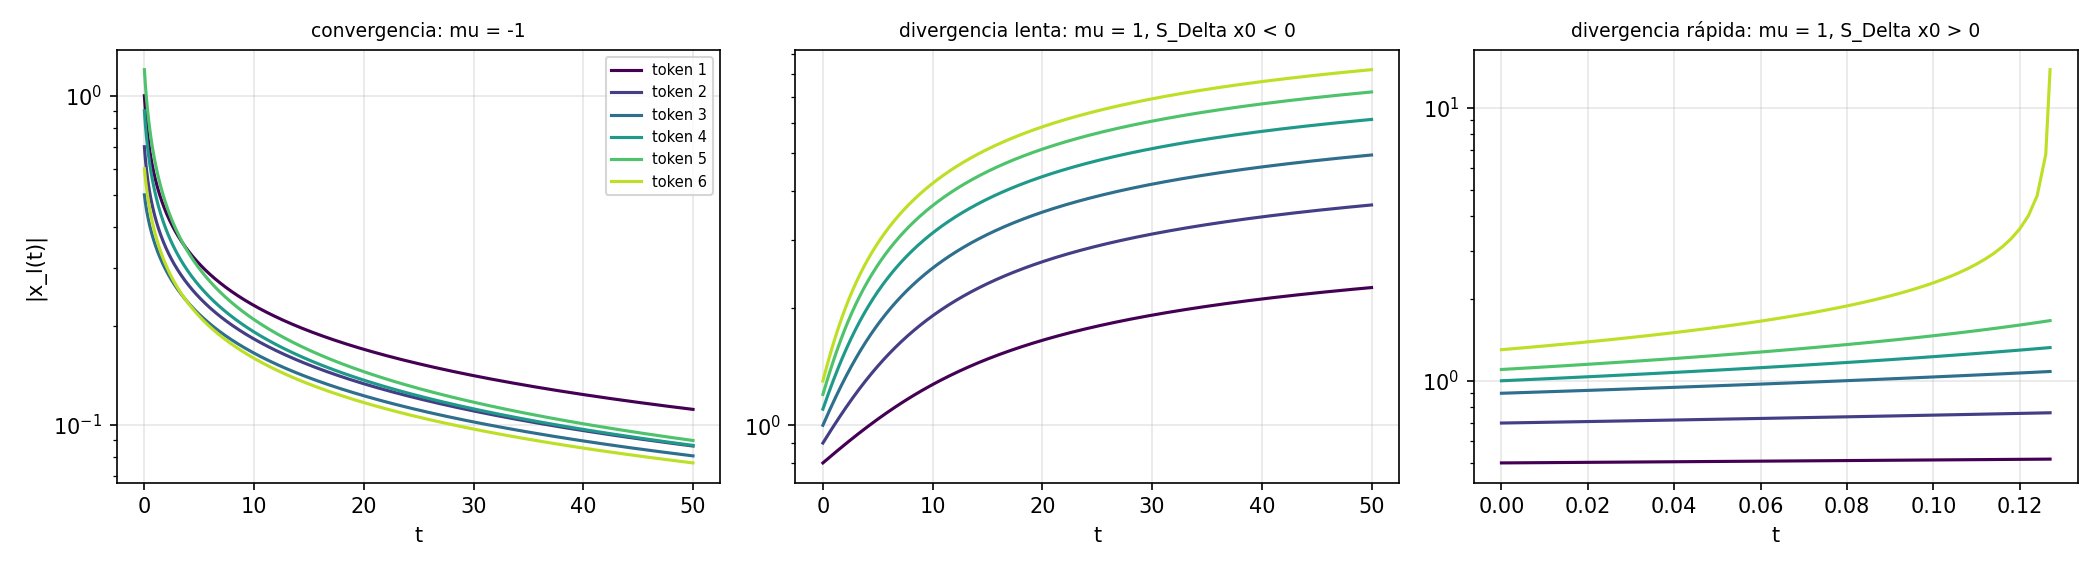
\includegraphics[width=\linewidth]{param_escenarios.png}
  \caption{Los tres escenarios del caso unidimensional: convergencia, divergencia lenta y divergencia rápida.}
  \label{fig:param-escenarios}
\end{figure}

\begin{figure}[t]
  \centering
  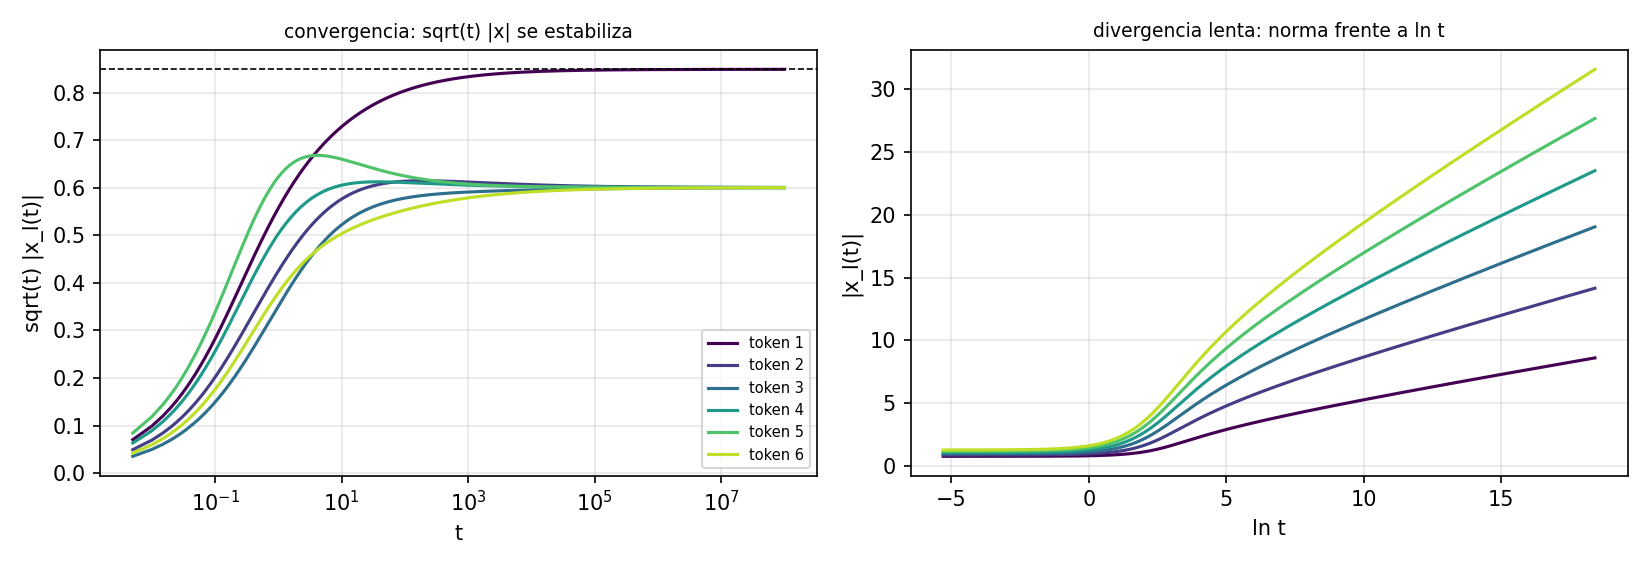
\includegraphics[width=\linewidth]{param_tasas_largas.png}
  \caption{Comprobación de las tasas del teorema a tiempos largos.}
  \label{fig:param-tasas}
\end{figure}

Los tres escenarios coinciden con la clasificación de la sección~\ref{sec:din-1d} (figura~\ref{fig:param-escenarios}). Con $\mu<0$ todos los tokens decaen y a $t=50$ cumplen $\lvert x_l\rvert\in[0.08,0.11]$. Con $\mu>0$ y $S_\Delta x_l(0)\le-2.12$ crecen sin explotar, hasta $\lvert x_l(50)\rvert\approx 2.3,\,3.7,\dots,8.2$ para $l=1,\dots,6$, y el crecimiento aumenta con la posición. Con $S_\Delta x_l(0)>0$ la solución explota en tiempo finito, aquí en $t\approx0.127$.

El parámetro $a$ cambia poco el comportamiento cualitativo (barridos no mostrados en figuras, disponibles en \texttt{figures/}). En convergencia solo desplaza el nivel de los tokens $l\ge2$: con $a=0.1$ valen $0.02$--$0.06$ a $t=50$ y con $a=5$ unos $0.11$--$0.13$, es decir, un $a$ grande aísla los tokens y cada uno evoluciona como si estuviese solo, de forma que su norma tiende a la del primer token ($0.111$). En divergencia lenta apenas hay diferencias ($\lvert x_6(50)\rvert$ pasa de $8.3$ a $7.8$). Algo parecido ocurre con $S_\Delta$ en convergencia: el primer token pasa de $0.115$ a $0.096$ al multiplicar $S_\Delta$ por~8. Ni $a$ ni $S_\Delta$ modifican, por tanto, el escenario; lo fija el signo de $\mu$ y el de $S_\Delta x_l(0)$.

Por último, comprobamos las tasas de la sección~\ref{sec:din-tasas} integrando hasta $t=10^8$ con paso proporcional a $t$ (figura~\ref{fig:param-tasas}). En convergencia la pendiente log-log de $\lvert x_l\rvert$ para $t>10^4$ es $-0.50$ en los seis tokens, igual a la del teorema~\ref{thm:din-conv}. En divergencia lenta, un ajuste $\lvert x_l\rvert\sim(\ln t)^{\beta}$ para $t>10^3$ da $\beta\approx0.8$ en todos los tokens, compatible con la cota $(\ln t)^l$ del teorema~\ref{thm:din-lenta}, que para $l=1$ ya vale $\beta\le1$. La cota no es ajustada para $l>1$: la simulación no muestra la dependencia en $l$ del exponente, aunque sí que el crecimiento es más rápido en los tokens posteriores.

\subsection{Longitud de secuencia y memoria de largo contexto}
\label{sec:sim-long}

\paragraph{Diseño.}
Se mide cuánta memoria del primer token conserva el último al crecer el número de tokens $L$, con dos medidas: el peso $\lvert P_{L1}\rvert$ y la sensibilidad $\lvert\partial x_L(T)/\partial x_1(0)\rvert$ (calculada con el método del paso complejo).
También se estudia cómo cambia el tiempo de explosión de la divergencia rápida con $L$. Se toman $L\in\{2,4,\dots,64\}$ y $a\in\{0.1,1,5\}$, con los parámetros de los tres escenarios anteriores, y se mide en $T=10$ (en la divergencia rápida, al $80\,\%$ del tiempo de explosión).

\begin{figure}[t]
  \centering
  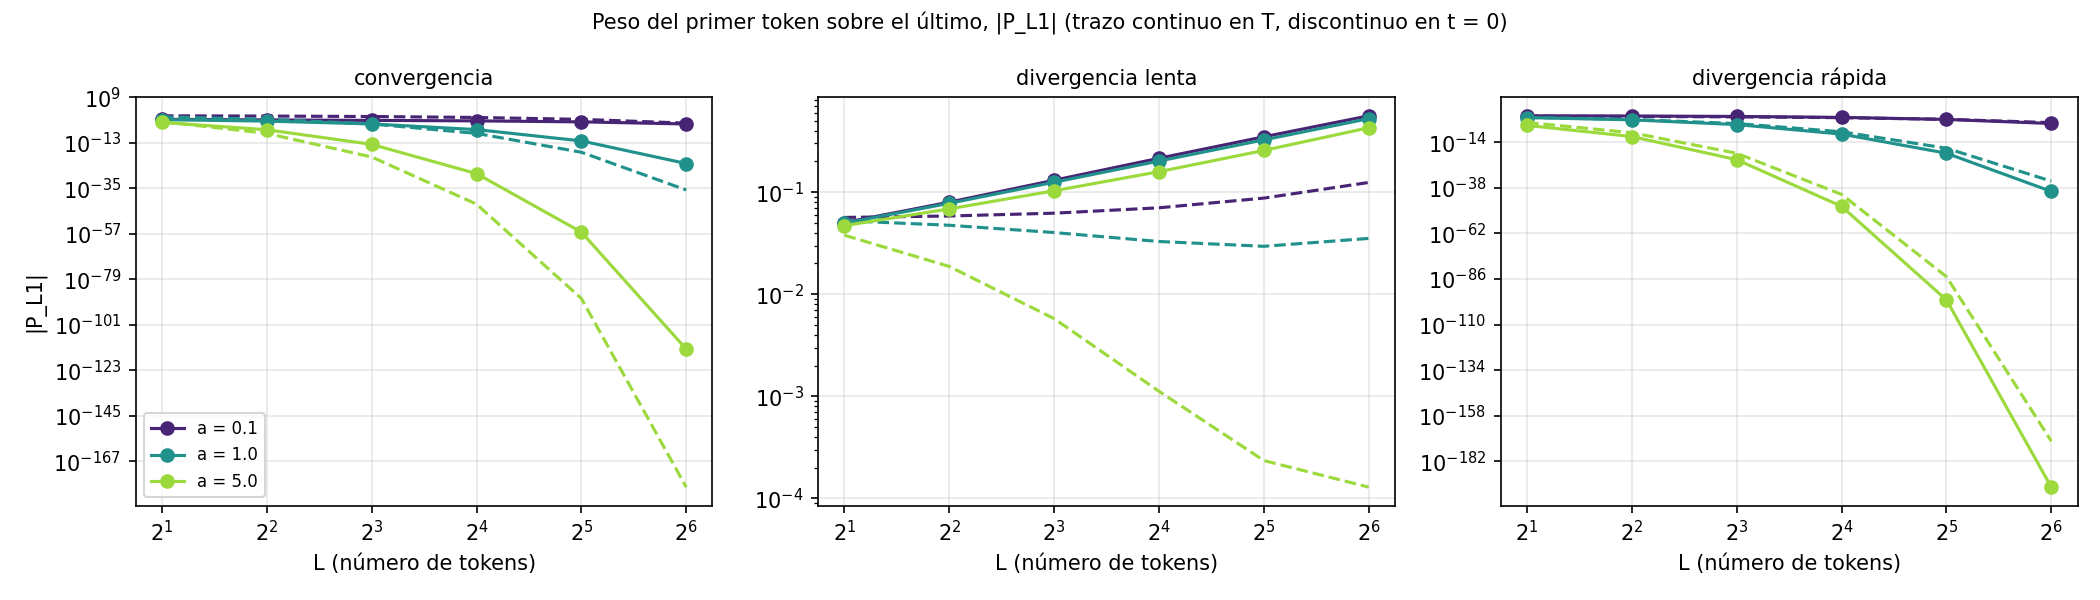
\includegraphics[width=\linewidth]{long_peso.png}
  \caption{Peso del primer token sobre el último, $\lvert P_{L1}\rvert$, frente a $L$.}
  \label{fig:long-peso}
\end{figure}

\begin{figure}[t]
  \centering
  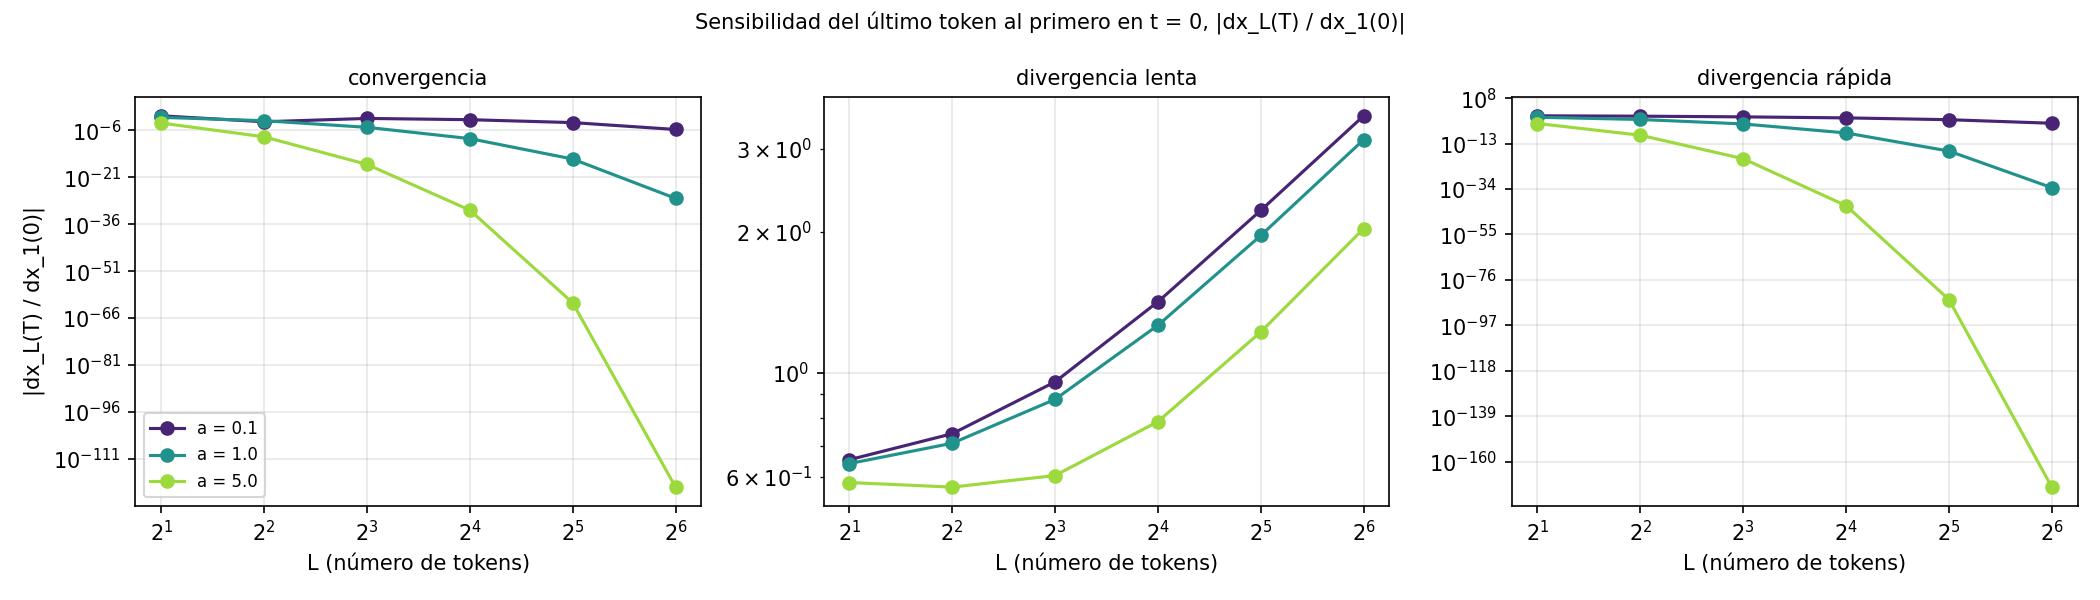
\includegraphics[width=\linewidth]{long_sensibilidad.png}
  \caption{Sensibilidad del último token al primero, $\lvert\partial x_L(T)/\partial x_1(0)\rvert$, frente a $L$.}
  \label{fig:long-sensibilidad}
\end{figure}

\emph{Convergencia.} La memoria se pierde al crecer $L$ y lo hace más deprisa cuanto mayor es $a$. Con $a=1$, la sensibilidad en $T=10$ baja de $1.4\cdot10^{-2}$ ($L=2$) a $2\cdot10^{-28}$ ($L=64$). La causa es el factor $\exp(-a\sum_{k=2}^{L}\Delta(x_k))$ de $P_{L1}$: como $\Delta(x_k)$ no se anula, la suma crece con $L$ (de $0.8$ a $50$ con $L=2,\dots,64$) y el decaimiento es exponencial en la longitud. Incluso con $a=0.1$ la sensibilidad cae de $4\cdot10^{-2}$ a $2\cdot10^{-6}$.

\emph{Divergencia lenta.} Es el único escenario en que el último token conserva información del primero. Los $\Delta(x_k)$ son casi nulos ($S_\Delta x_k\le-2.4$), así que $\sum_k\Delta(x_k)$ satura por debajo de $10^{-2}$ y el factor exponencial queda $\approx1$ para cualquier $L$ y $a$. De ahí que $\lvert P_{L1}\rvert$ en $T=10$ crezca con $L$ (de $0.05$ a $0.5$ con $a=1$) y también la sensibilidad (de $0.64$ a $3.1$). Debe leerse con cuidado: es un resultado a tiempo finito, y el teorema~\ref{thm:din-lenta} da $P_{lj}\to0$ cuando $t\to\infty$, de modo que la memoria es transitoria aunque la sensibilidad siga creciendo.

\emph{Divergencia rápida.} Con $a\ge1$ la memoria se destruye antes que en convergencia ($\lvert P_{L1}\rvert\sim10^{-40}$ con $a=1$ y $L=64$, y $\sim10^{-196}$ con $a=5$), porque aquí $\sum_k\Delta(x_k)\approx 90$ con $L=64$. Con $a=0.1$ decae más despacio, pero sigue siendo pequeña ($8\cdot10^{-5}$). El tiempo de explosión baja con $L$ solo si $a$ es pequeño ($0.13\to0.03$ con $a=0.1$; $0.137\to0.119$ con $a=1$) y es independiente de $L$ ($0.138$) con $a=5$, porque los tokens quedan desacoplados y explota por sí solo el de mayor valor inicial ($1.3$), que es el mismo para todo $L$.

En resumen, en ninguno de los escenarios que entran en la clasificación de la sección~\ref{sec:din-1d} se conserva memoria de largo contexto de forma sostenida: solo la divergencia lenta la mantiene en un horizonte finito.


\newpage
% ============================================================================
% 5. Tabla comparativa SSM selectivo vs. self-attention
% Responsable: \todo{decidir: la persona que NO escribe la introducción}
% Prefijo de etiquetas: sec:comparacion, tab:comp-, fig:comp-
% ============================================================================
\section{Comparación con self-attention}
\label{sec:comparacion}

\todo{Texto introductorio y tabla. Criterios sugeridos: coste computacional en $L$, memoria, forma de la dinámica de tokens, tipo de colapso, qué lo controla.}

\begin{table}[t]
  \centering
  \caption{Comparación entre SSM selectivo y self-attention.}
  \label{tab:comp-ssm-attention}
  \begin{tabular}{lll}
    \toprule
    Criterio & SSM selectivo (Mamba) & Self-attention \\
    \midrule
    \todo{criterio} & \todo{} & \todo{} \\
    \bottomrule
  \end{tabular}
\end{table}

\newpage
% ============================ 6. Conclusiones ============================
\section{Conclusiones}
\label{sec:conclusiones}


\newpage

% ====================== BIBLIOGRAFÍA ===========================
\section{Referencias}
\printbibliography

% ====================== ANEXOS ===========================
% \appendix
% \input{sections/.tex}

\end{document}
